\chapter{Directional Sound Separation}\label{ch:directional}
This chapter deals with directional filtering. In the beginning, the prerequisites for 
the filtering idea are presented. Afterwards, the actual filtering idea is shown and explained.
In the end, the results are presented, and a conclusion is drawn.
\section{Concept}
Figure \ref{fig:2sources} shows a scenario where directional filtering could be used.
Source 1 and Source 2 are both talking simultaneously. At the origin, two microphones,
left (L) and right (R) are fixed and recording.

\begin{figure}[htp]
	\centering
	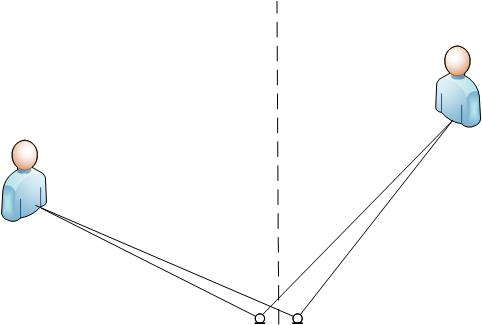
\includegraphics[width=0.65\textwidth]{Illustrations/2sources.jpg}
	\caption{Two Persons Talking}
	\label{fig:2sources}
\end{figure}

Due to the nature of the setup, the microphones will record  both the speakers.
However, both microphones record two persons talking. As a consequence, each microphone
returns a soundwave containing two signals. The aim is to filter out one of them
by only using the two soundwaves available.

In order to be able to do this, one assumption needs to be made. That is, that the 
angle at which each source is located, is known.

\begin{figure}[htp]
	\centering
	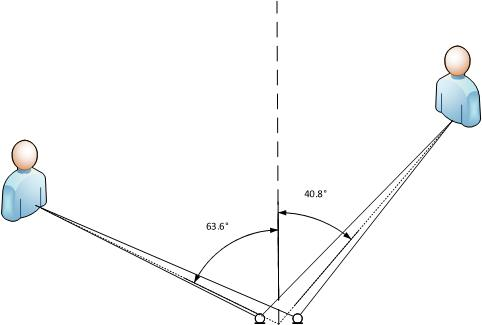
\includegraphics[width=0.67\textwidth]{Illustrations/2sourcesWangles.jpg}
	\caption{Two Persons Talking With Known Angles}
	\label{fig:2sourcesWangles}
\end{figure}

Figure \ref{fig:2sourcesWangles} represents the same scenario. However this time, the angles
of the sound sources are known. The Sources and the Origin are represented with coordinates.
This helps in determining the formulas that are needed in order to obtain the delay in samples.

\begin{figure}[htp]
	\centering
	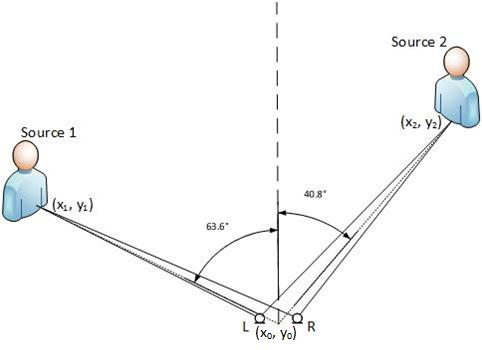
\includegraphics[width=0.67\textwidth]{Illustrations/2sourcesWanglesAndPossition.jpg}
	\caption{Two Persons Talking With Known Angles}
	\label{fig:2sourcesWanglesAndPossition}
\end{figure}

\newpage

Figure \ref{fig:zoomedin1} represents the delay between the two signals. One advantage
is represented by the fact that, no matter the distance of the source, the delay between the
signals is always the same. The delay in samples is only dependent on the distance between the mics.
By knowing the angle, the sampling frequnecy and the travelling speed of sound, the delay in 
samples can be determined. By increasing the distance between the microphones, greater accuracy 
could be obtained. However this would also result in a bigger difference in terms of signal gain.
One signal would be significantly louder than the other to the point where filtering would not work.


\begin{figure}[htp]
	\centering
	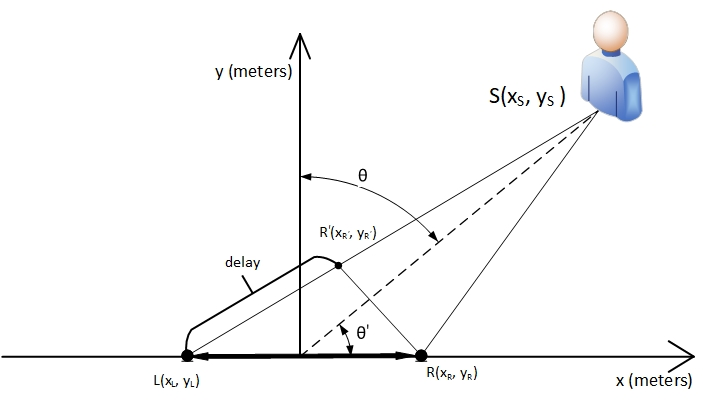
\includegraphics[width=0.65\textwidth]{Illustrations/delayDrawingForEquations.jpg}
	\caption{Delay}
	\label{fig:zoomedin1}
\end{figure}

\newpage
\section{Mathematical Solution}

Figure \ref{fig:zoomedin2} is a simplified version of Figure \ref{fig:zoomedin1} in order to better
understand the mathematical proof of finding the delay in number of samples.
\begin{figure}[htp]
	\centering
	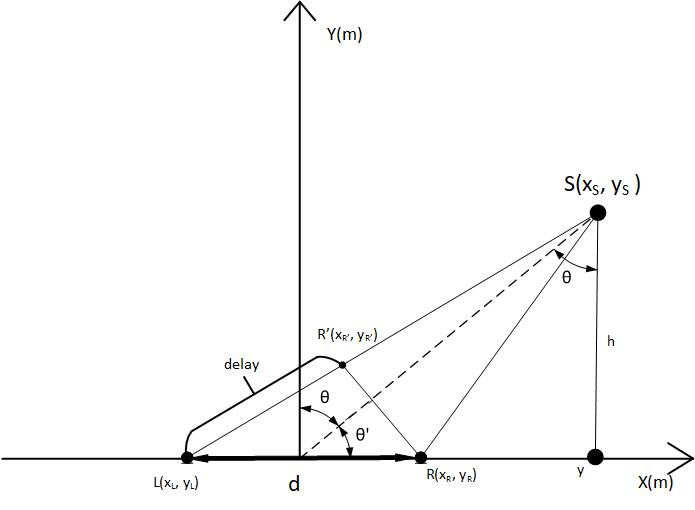
\includegraphics[width=1\textwidth]{Illustrations/mathematicalShit.jpg}
	\caption{Mathematical Interpretation}
	\label{fig:zoomedin2}
\end{figure}

Firstly, the distances SR and SL must be determined. This can be found by employing 
basic trigonometry. This is done by independently finding out the sides of the triangles
SyL  and SyR.

\begin{equation}
	yR = sin(\theta) - \dfrac{d}{2} 
\end{equation}

\begin{equation}
	yL = sin(\theta) + \dfrac{d}{2}
\end{equation}

After the x-coordinates are determined, h is needed in order to calculate the y-coordinates.

\begin{equation}
	h = cos(\theta)
\end{equation}

\newpage
Lastly, the sides SR and SL are determined.

\begin{equation}
	SR = \sqrt{h^2 + yR^2}
\end{equation}

\begin{equation}
	SL = \sqrt{h^2 + yL^2}
\end{equation}

Once the distances are known, the difference in distance between the signals can be found.

\begin{equation}
	delay = SL - SR
\end{equation}

At this moment, the delay is expressed in distance. By knowing the speed of sound, the amount of
time it takes to travel that distance can be found.

\begin{equation}
	delayInTime = \frac{delay}{speed of sound}
\end{equation}

The time, can be converted in amount of samples by multiplying it by the sampling frequency.

\begin{equation}
	delayInSamples = delayInTime * SamplingFrequncy
\end{equation}

\newpage
\section{Filtering Idea}
With the angles of both sources known, one or the other source can be isolated. The only 
sound source considered in this project was human voice. Therefore, the aim is to 
separate the two voices, by only using the sound samples recorded by both microphones. 
The data recorded by each microphone, contains two separate human speeches.
Figure XX explains the process. Afterwards, a more visual example will be discussed,
aimed at better describing the procedure. 

\begin{figure}[htp]
	\centering
	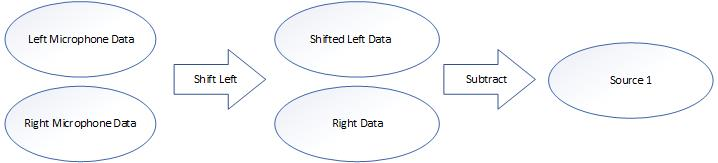
\includegraphics[width=1\textwidth]{Illustrations/IdeaDiagram.jpg}
	\caption{Idea diagram}
	\label{fig:IdeaDiagram}
\end{figure}

\todo[inline]{redo diagram}

Both microphones record the same data. The only two differences, are the delay in time,
and the gain difference. By shifting one recorded sample in order to match the other,
and subtracting the signals, the matched data is eliminated. This means that by aligning 
one speech, and then subtracting, the other speech is separated and obtained.

\newpage

\section{Visual Example}
A visual example is explained below. Actual differences can even be seen on the waveforms themselves.
The example is ideal, meaning there is no noise applied to the signals, and their purpose is to 
prove the idea.

\begin{figure}[htp]
	\centering
	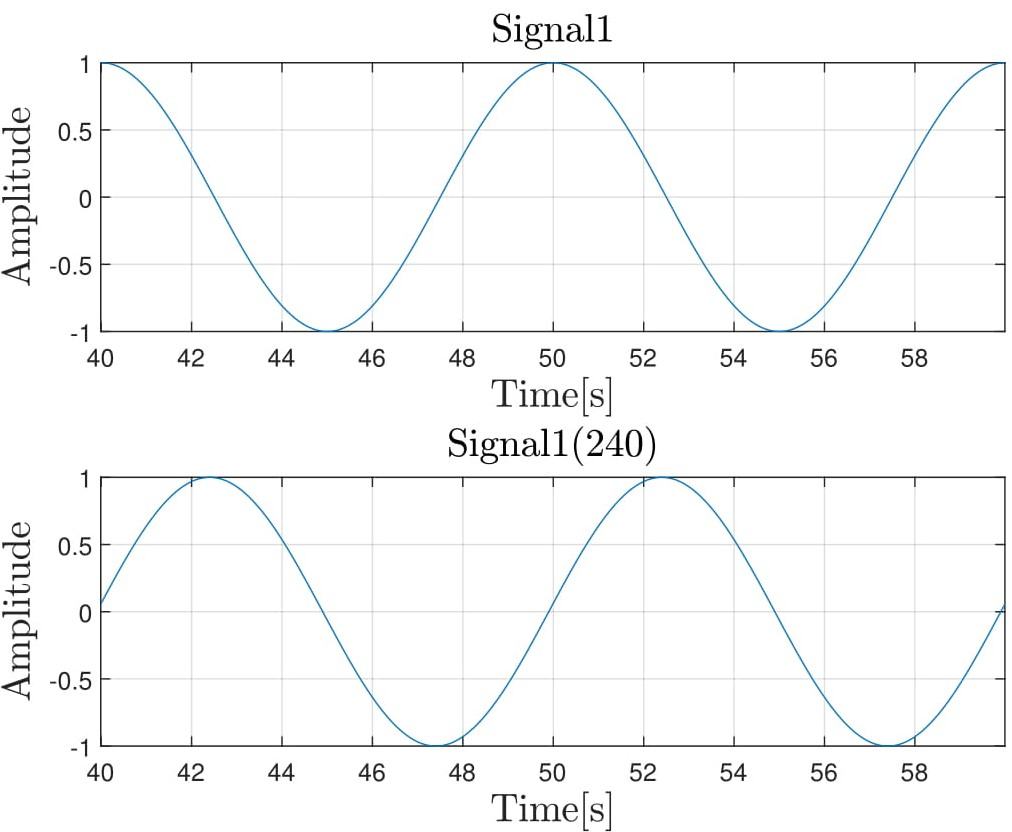
\includegraphics[width=\textwidth]{Illustrations/source1.jpg}
	\caption{First Source}
	\label{fig:source1}
\end{figure}

Figure \ref{fig:source1} shows a simple sine wave. Source 1 is the original signal. Source 1-Right Shifted
is the same signal just shifted to the right by 240 samples.

\newpage

Figure \ref{fig:source2} shows another sine wave, with a higher frequency and a lower amplitude. This 
represents the second source. Source 2 is the original signal. Source 2 - Left Shifted is the same signal
shifted to the left by 377 samples.


\begin{figure}[htp]
	\centering
	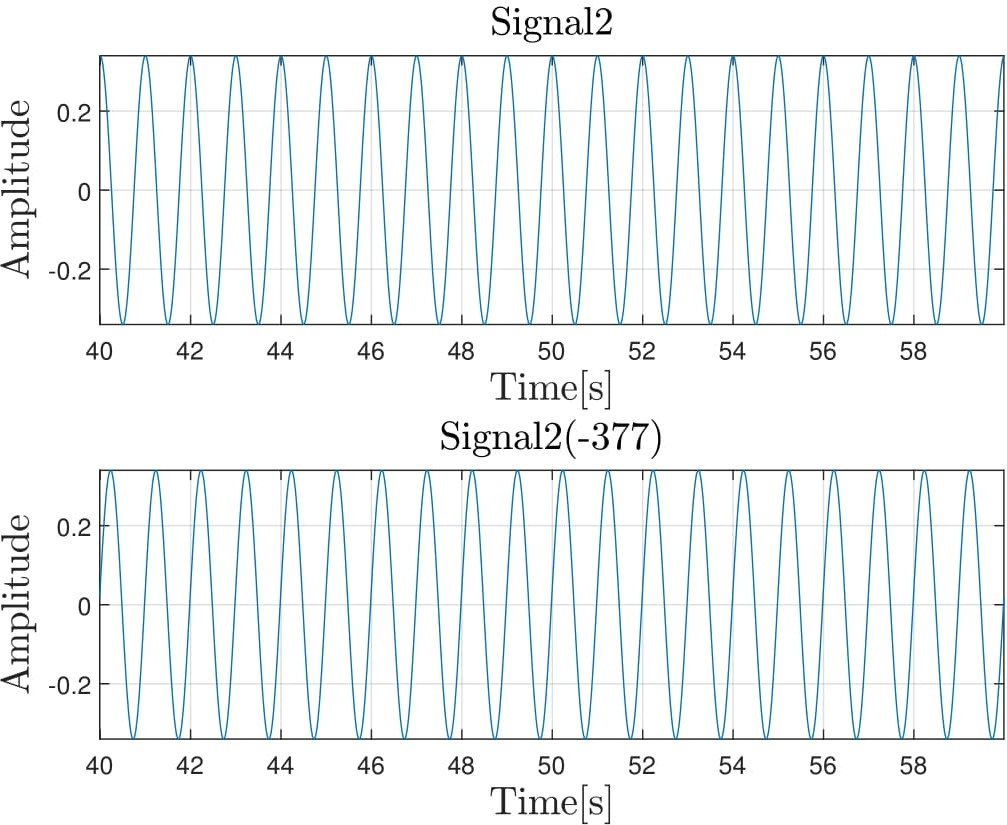
\includegraphics[width=\textwidth]{Illustrations/source2.jpg}
	\caption{Second Source}
	\label{fig:source2}
\end{figure}
Next step involves adding the signals.
\begin{equation}
	Source1 + Source2LeftShifted = LeftMicrophone
	\label{eq:leftMicrophone}
\end{equation}


\begin{equation}
	Source1RightShifted + Source2 = RightMicrophone
	\label{eq:rightMicrophone}
\end{equation}

Equations \ref{eq:leftMicrophone} and \ref{eq:rightMicrophone} now have both signals from both sources.
\newpage
$LeftMicrophone$ contains $Source1$ and $Source2LeftShifted$. $RightMicrophone$ contains $Source2$
and $Source1RightShifted$.
\begin{figure}[htp]
	\centering
	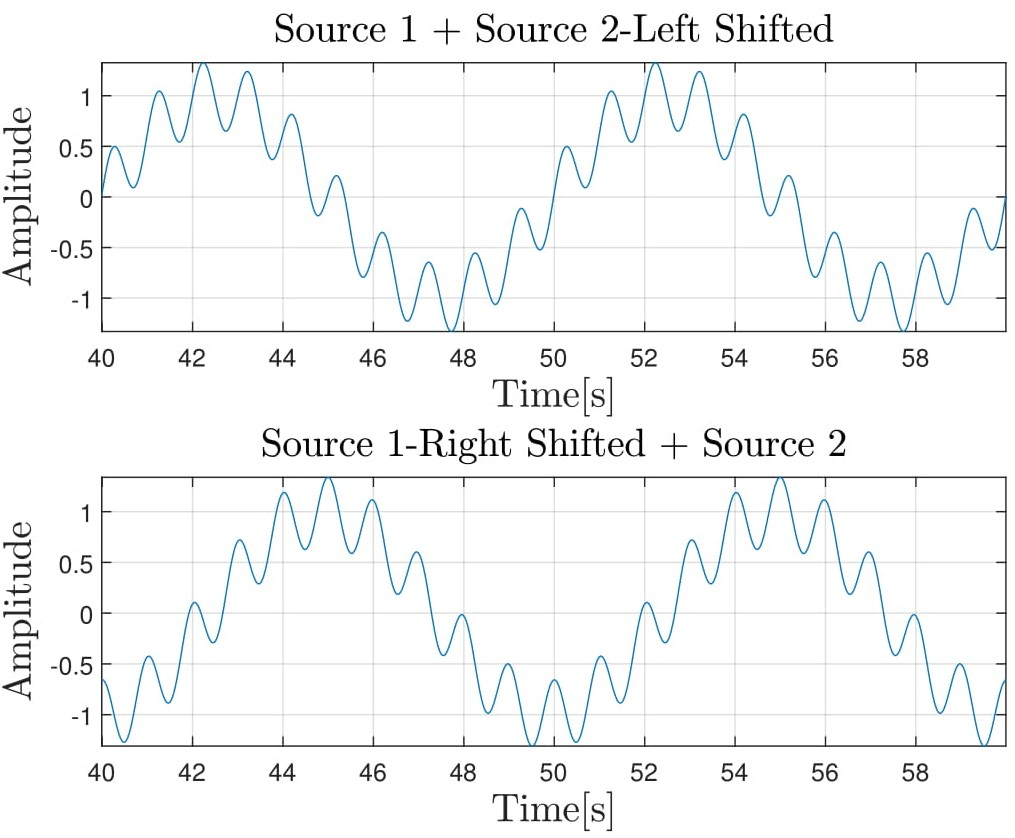
\includegraphics[width=\textwidth]{Illustrations/source1And2.jpg}
	\caption{Added Signals}
	\label{fig:source1And2}
\end{figure}

They are represented in Figure \ref{fig:source1And2}. The summation of both signals can clearly 
be seen above.
\newpage
\subsection*{Sound Separation}
We aim at separating the sounds by only using the previous signals seen in Figure \ref{fig:source1And2}.
Knowing the angles and the amount of delay in samples, the separation of the two signals reduces to
a matter of matching and subtracting them. 

Important to notice. The matched signal is the one filtered out.
\begin{figure}[htp]
	\centering
	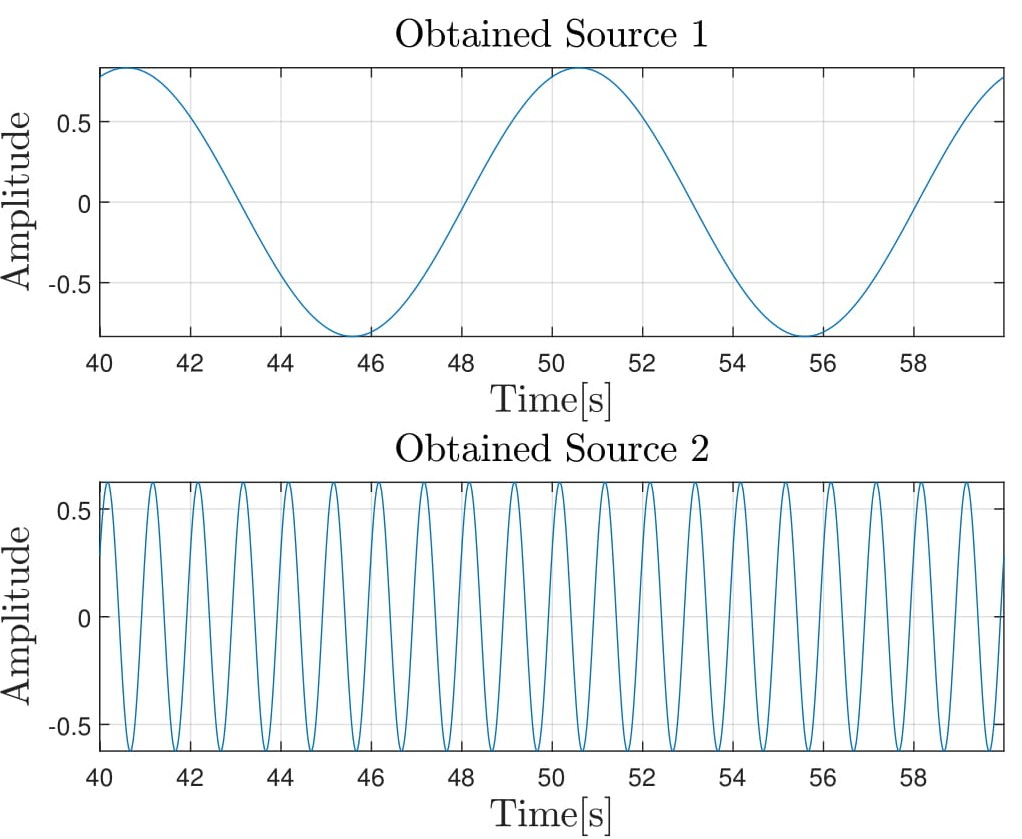
\includegraphics[width=0.8\textwidth]{Illustrations/obtainedSource1And2.jpg}
	\caption{Obtained Signals}
	\label{fig:obtainedSignals}
\end{figure}

\subsection*{Observations}
The signals seem to have a slight phase shift. Additionally, they have higher amplitudes, than the original
signals. As of right now, we are not able to determine why. However the waveforms are very similar.
All figure can be seen in Appendix X.
\todo[inline]{remember to put stuff in appendix}
\newpage

\section{Filtering}
All of the directional filtering is done by applying the logic discussed before to the Matlab script.\\
Prior to shifting signals and filtering, we had to remove any delays, induced by hardware or software. This 
issue was resolved by starting every recording with loud, sharp sound like a clap or a finger snap right in 
the middle of the microphones. Using this sound in the beginning we could match loudest peaks, thus 
eliminating hardware and software induced delay. \\
\subsection{One sound source}
To see if we can get the samples, which show that logic behind direction of delay is correct, we set up a 
recording with just one person first see figure \ref{fig:RanzvanRecSetup}.


Then we looked at collected data:\\
When person spoke from the center, (Figure \ref{fig:C}) shows that recordings match in phase. Green graph is 
data, captured by left microphone and yellow graph is data, captured by right microphone.
\begin{figure}[htp]
  \centering
  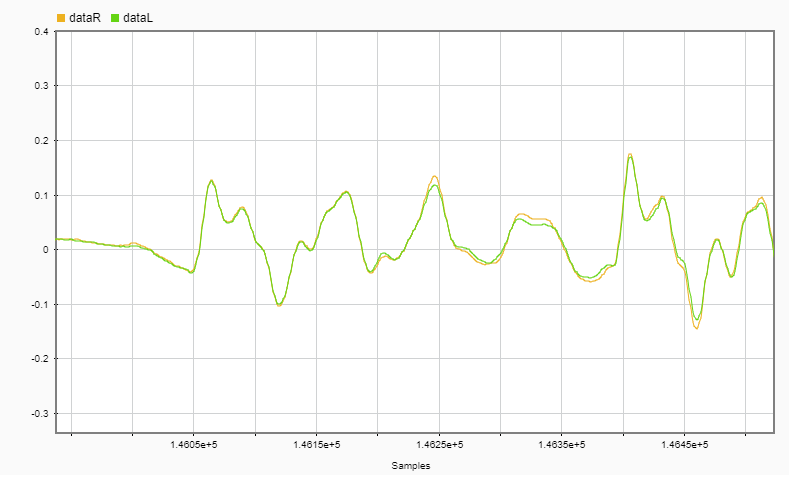
\includegraphics[width=0.75\linewidth]{Illustrations/DataC.png}
  \caption{Data from speaker in the center}
  \label{fig:C}
\end{figure}

When person spoke from the right, right microphone data led left microphone (Figure \ref{fig:R}), here blue graph is left microphone data and orange graph represents right microphone data.\\
\begin{figure}[htp]
  \centering
  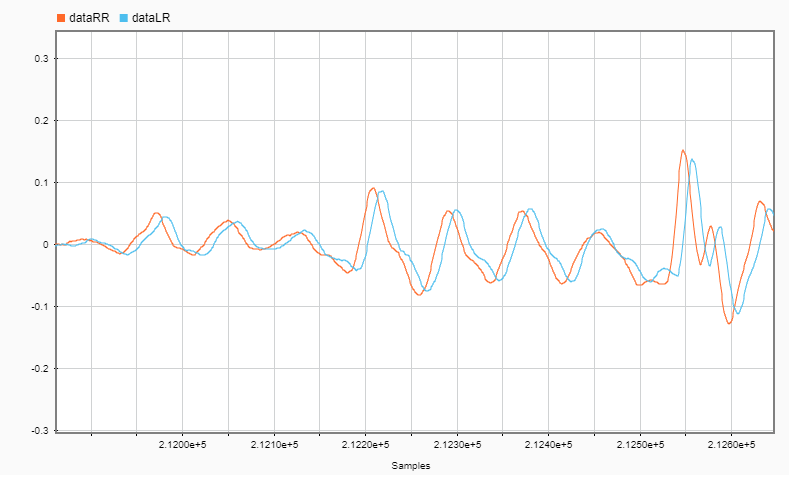
\includegraphics[width=0.75\linewidth]{Illustrations/DataR.png}
  \caption{Data from speaker in the right side}
  \label{fig:R}
\end{figure}

When he spoke from the left, left microphone was leading the right (Figure \ref{fig:L}) pink graph is left microphone data and purple graph shows right microphone data.
\begin{figure}[htp]
  \centering
  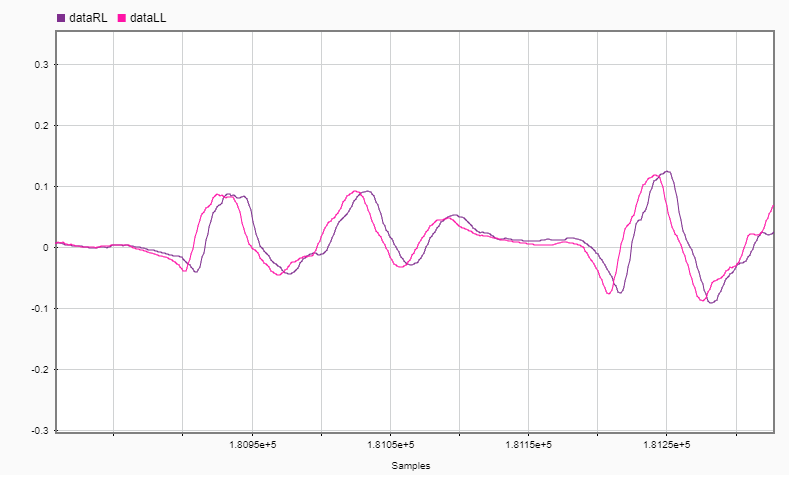
\includegraphics[width=0.75\linewidth]{Illustrations/DataL.png}
  \caption{Data from speaker in the left side}
  \label{fig:L}
\end{figure}

All of the directional filtering is done by applying the logic discussed in the Idea for filtering section to 
the Matlab script.\\
First we took data from the recording with only one person, shifted left microphone to match right microphone 
data in phase, then subtracted right microphone data from shifted left microphone data - got "Separated" signal.\\
After re-listening the separated signal from this filtering process, separated signal contained enough data to 
still hear what the person was saying even though the goal was to hear relative silence, sound level dropped 
significantly. This can be seen in figure \ref{fig:oneSourceSepAndOG}.

\begin{figure}[htp]
  \centering
  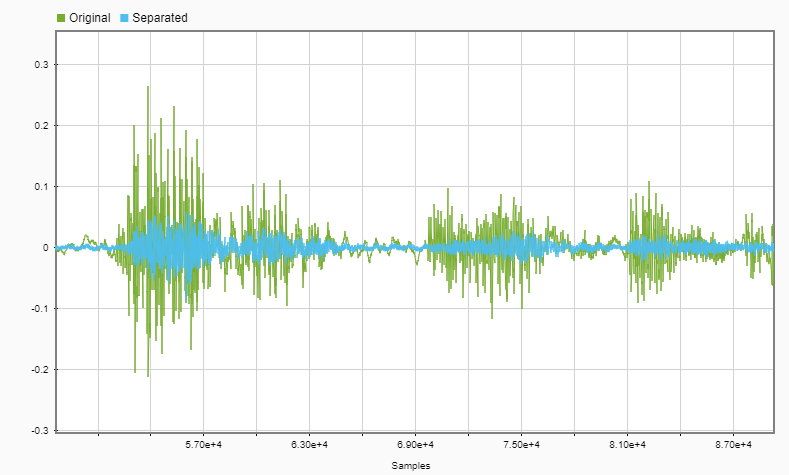
\includegraphics[width=0.7\linewidth]{Illustrations/OnePersonOriginalAndSeparated.png}
  \caption{Data comparison of separated and original signals of one person talking}
  \label{fig:oneSourceSepAndOG}
\end{figure}

\subsection{Two sound sources}
When we saw a significant decrease of sound level, but we could still hear what was going on, we assumed, that it 
might be because of no other sounds were present and when we get two sources, the one we opt to hear will be loud 
enough in comparison for separation to work. So we applied the same process to the samples we got from two people 
talking at the same time as to what we did with only one person talking.\\

After shifting left microphone we could see some data line up with the right microphone data in figure 
\ref{fig:2sourcesShifted}., which seems like it could work and it would separate the unwanted sounds from the samples. 

\begin{figure}[htp]
  \centering
  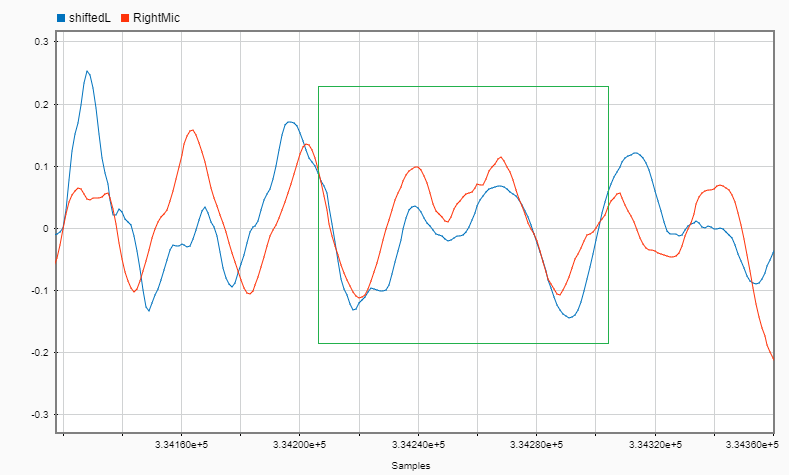
\includegraphics[width=0.7\linewidth]{Illustrations/twoSourcesShiftedandOriginal.png}
  \caption{Two sources at the same time, in the graph: shifted left microphone data and right microphone data}
  \label{fig:2sourcesShifted}
\end{figure}

Then we compared output data to original data (see figure \ref{fig:2sourcesSeparated} and not many visual 
differences were seen as well. Also, when listening to the output, we couldn't hear any audible difference from 
the original sample either.

\begin{figure}[htp]
  \centering
  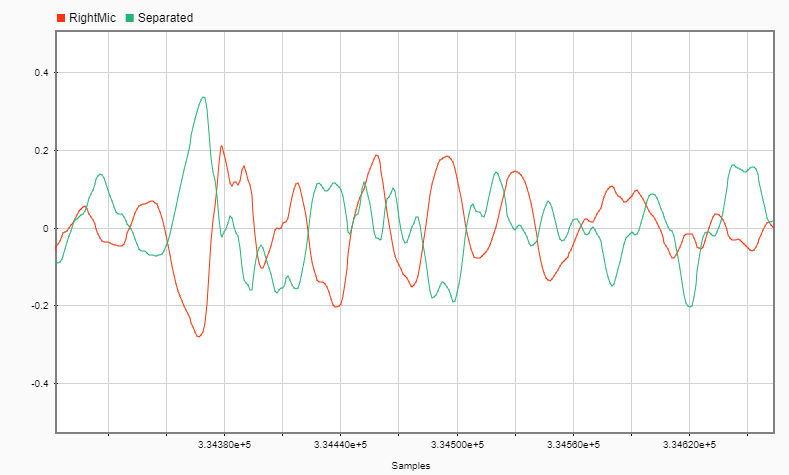
\includegraphics[width=0.7\linewidth]{Illustrations/twoSourcesSeparatedandOriginal.png}
  \caption{Two sources at the same time, in the graph: separated signal data and right microphone data}
  \label{fig:2sourcesSeparated}
\end{figure}
We considered this a failed attempt, but not because of the method, rather because of the 
equipment used, which was not ideal - both of the microphones didn't capture the sound waves 
identically. This can be seen when we do loud clap directly in the center of the microphones. 
Ideally, microphones would register identical waveform, but in the figure \ref{fig:clap} we can 
see that the sound wave of a clap is registered a bit differently by right and left 
microphones.
\begin{figure}[htp]
  \centering
  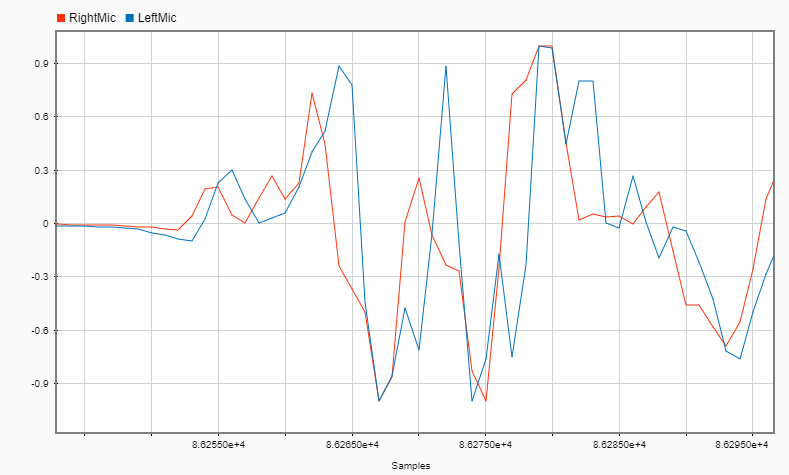
\includegraphics[width=0.7\linewidth]{Illustrations/clap.png}
  \caption{Clap in the beginning of recording}
  \label{fig:clap}
\end{figure}

\section{Synthetic Samples}
  Because we couldn't get any visible or audible results with our filtering method of real recordings with two 
microphones and one sound source and it was even worse with two sound sources at the same time, we have 
decided to try recording each person separately, using one microphone and then synthetically articulate data, 
as if we recorded two sound sources at the same time to two microphones by adding delay and gain on both 
sources which made it look and sound realistically.\\
  In order to create samples to sound as realistic as possible we had to look in delay differences as well as 
gain loss over distance. \\
Using synthetic samples also gives us more flexibility when testing the code, we just need to adjust the 
angle that we want to place sources at. 
  \subsection{Gain ratio}
  Code for making synthetic samples needs angles that we want to place sources at and the gap between the 
microphones. For shifting we can use code we did to calculate shift in delays from a given angle. Shift the signal 
and then add gain ratio. \\
  Relationship of sound strength is what we call gain ratio. Sound strength falls by a ratio of \( \frac{1}{2}
\) when the distance is doubled. Which means that sound strength follows distance inverse-proportionally. 
  By giving one of the microphones gain ratio of 1 we can calculate what is the ratio for the other 
microphone. Figure \ref{fig:ratioDependence} illustrates the variables used in the equations.
\begin{figure}[htp]
	\centering
	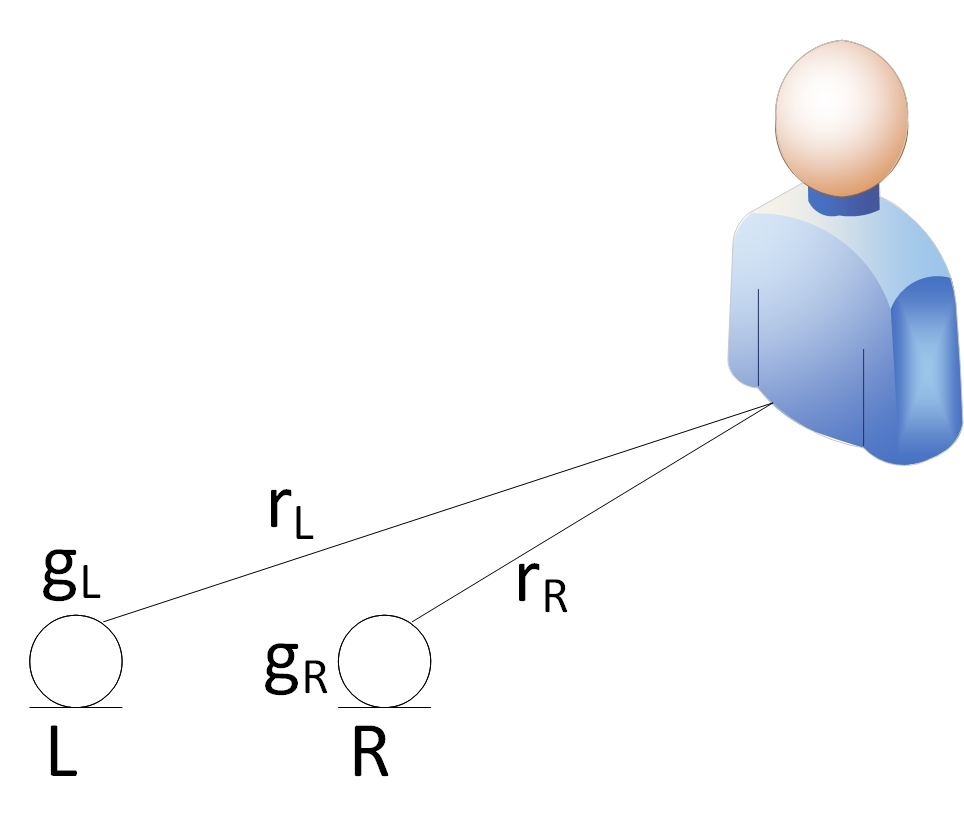
\includegraphics[width=0.35\textwidth]{Illustrations/gainRatio.jpg}
	\caption{Gain ratio dependence on distance}
	\label{fig:ratioDependence}
\end{figure}
 \[\frac{r_L}{r_R} = \frac{dist_R}{dist_L} \]\\
Using this proportion and keeping \(r_L\) as 1 we can calculate gain \(r_R\), which we will multiply with 
right microphone data to get realistic gain loss. Distances \(dist_L\) and \(dist_R\) here are the same 
distances, which we calculate in delay code. This means that in order to get the gain ratio for right 
microphone we just need to divide distance to the left microphone (\(dist_L\)) by distance to the right 
microphone (\(dist_R\)).
\subsection{Adding recordings}
First, audio recordings of sources are made the same size. Then parts of each source, which will go to the left 
microphone are shifted according to the angle, we want to put that source at. Then, the part, which will go to the 
right microphone is multiplied with gain ratio \(r\). The same is done with all of the sources we use. In the end, 
all of the left and right microphone assigned sources will be summed to left microphone data and right microphone 
data. 


 

\section{Conclusion}